\chapter{About Dresden OCL}
\label{chapter:about}

\begin{flushright}
\textit{Chapter written by Claas Wilke and Michael Thiele}
\end{flushright}

\emph{DresdenOCL} is developed as a project at the Technische Universit�t Dresden (TUD), Software Technology Group since 1999. Its latest version is released as a set of Eclipse plug-ins and thus, called \emph{\acl{DOT4Eclipse}}. DresdenOCL contains a set of OCL tools, including an OCL parser, an OCL interpreter and an OCL-to-Java code generator.

In this chapter, some general information on DresdenOCL is presented. The supported OCL version and the differences to the official OCL specification are documented. Supported meta-models, models and model instances are shortly presented. If you are not interested in such information, you can skip this chapter and continue with the installation and general use of DresdenOCL as documented in Chapter \ref{chapter:introduction}.
  


\section{Supported Version of OCL}

DresdenOCL generally supports OCL 2.2 as specified in \cite{spec:OCL2-2}. Nevertheless, some differences between DresdenOCL and OCL 2.2 exist as documented in the following:


\subsection{Missing Features of OCL 2.2 in DresdenOCL}

\begin{itemize}
	\item Currently, the OCL keywords \code{static}, \code{null} and \code{invalid} are not supported but will be supported by the next released version of DresdenOCL (version 2.3).
	\item Messages as defined in the OCL 2.2 specification are not supported by DresdenOCL. They can neither be parsed, nor interpreted, nor can code be generated for messages.
\end{itemize}
	
	
\subsection{Different Semantics of OCL Expressions in DresdenOCL}

The current OCL 2.2 specification \cite{spec:OCL2-2} contains some inconsistencies and misses some definitions especially when evaluating \code{invalid} or \code{null} values. Thus, we had to assume or change the semantics of OCL during interpretation of some OCL statements. In the following we present the differences of the OCL semantics used in DresdenOCL compared with the official OCL specification \cite{spec:OCL2-2}.


\subsubsection{Boolean Operators}

\begin{table}
	\centering
		\begin{tabular}{|p{1.2cm}p{1.2cm}||p{1.2cm}|p{1.2cm}|p{1.2cm}|p{1.2cm}|p{2.0cm}|}
			\hline
      \textbf{a}	& \textbf{b}	& \textbf{not a}	& \textbf{a or b}	& \textbf{a xor b} 	& \textbf{a and b}	& \textbf{a implies b} \\
			\hline
			false				&	false				&	true						&	false						& false							&	false							&	true \\
			\hline	
			false				&	true				&	-								&	true						& true							&	false							&	true \\
			\hline
			false				&	null				&	-								&	invalid					& invalid						&	false							&	true \\
			\hline
			false				&	invalid			&	-								&	invalid					& invalid						&	false							&	true \\
			\hline
			true				&	false				&	false						&	true						& true							&	false							&	false \\
			\hline
			true				&	true				&	-								&	true						& false							&	true							&	true \\
			\hline
			true				&	null				&	-								&	true						& invalid						&	invalid						&	invalid \\
			\hline
			true				&	invalid			&	-								&	true						& invalid						&	invalid						&	invalid \\
			\hline
			null				&	false				&	invalid					&	invalid					& invalid						&	false							&	invalid \\
			\hline
			null				&	true				&	-								&	true						& invalid						&	invalid						&	invalid \\
			\hline
			null				&	null				&	-								&	invalid					& invalid						&	invalid						&	invalid \\
			\hline
			null				& invalid			&	-								&	invalid					& invalid						&	invalid						&	invalid \\
			\hline
			invalid			& false				&	invalid					&	invalid					& invalid						&	false							&	invalid \\
			\hline
			invalid			&	true				&	-								&	true						& invalid						&	invalid						&	invalid \\
			\hline
			invalid			&	null				&	-								&	invalid					& invalid						&	invalid						&	invalid \\
			\hline
			invalid			&	invalid			&	-								&	invalid					& invalid						& invalid						&	invalid \\
			\hline
		\end{tabular}
		\caption{Decision Table for boolean operators in Dresden OCL.}
		\label{tab:decisionTable}
\end{table}

Boolean operators in DresdenOCL are interpreted as documented in Table \ref{tab:decisionTable}. As documented, the operator \code{and} always results in \code{false} as long as one of its operands is \code{false}, ignoring whether the other operand is \code{null} or even \code{invalid}. The operator \code{or} results in \code{true}, as long as one of its operands is \code{true}. Both \code{false implies null} and \code{false implies invalid} result in \code{true}. The operator \code{xor} can only be evaluated if both arguments are nor \code{null} nor \code{invalid}. Otherwise the operand will result in \}


\subsubsection{Equality in DresdenOCL}

\begin{table}
	\centering
		\begin{tabular}{|p{1.2cm}p{1.2cm}||p{1.2cm}|p{1.2cm}|p{1.2cm}|p{1.2cm}|p{1.2cm}|p{1.2cm}|}
			\hline
      \textbf{a} 	& \textbf{b} 	& \textbf{a = b} 	& \textbf{a <> b} 	& \textbf{a < b} 	& \textbf{a <= b} 	& \textbf{a > b} 	& \textbf{a >= b} \\
			\hline
			42					&	42					&	true						&	false							&	false						&	true							&	false							&	true \\
			\hline
			42					&	7						&	false						&	true							&	false						&	false							&	true							&	true \\
			\hline
			42					&	null				&	false						&	true							&	invalid					&	invalid						&	invalid						&	invalid \\
			\hline
			null				&	null				&	true						&	false							&	invalid					&	invalid						&	invalid						&	invalid \\
			\hline
			42					&	invalid			&	false						&	true							&	invalid					&	invalid						&	invalid						&	invalid \\
			\hline
			invalid			&	invalid			&	true						&	false							&	invalid					&	invalid						&	invalid						&	invalid \\
			\hline
		\end{tabular}
		\caption{Decision Table for equality operators in Dresden OCL.}
		\label{tab:info:equalityDecisionTable}
\end{table}

\acs{OCL} defines the two operators \code{=} and \code{<>} to compute equality of two given \acs{OCL} expressions. Since \acs{OCL} values can be both \code{null} or \code{invalid}, it is important to know how these operators behave when used with \code{null} and \code{invalid} values. According to the specification, comparing two \acs{OCL} values results in an illegal state when one of the two values is either \code{null} or \code{invalid}. However, it is not specified if the comparison results in \code{null} or \code{invalid} \cite[p. 195]{spec:OCL2-2}. In some situations this can lead to problems during evaluation, e.g., when iterating on an \acs{OCL} collection containing \code{null} values. 

Thus in DresdenOCL, using the operators \code{=} and \code{<>} for comparison will always result in \code{true} or \code{false} as documented in Table~\ref{tab:info:equalityDecisionTable}. But please be aware, that this behaviour is only implemented for \code{=} and \code{<>}. Using other comparison operators such as \code{<}, \code{<=}, \code{>}, and \code{>=} for numeric values can result in \code{invalid}!


\subsubsection{Collections}

In DresdenOCL, collections can contain \code{null} values but cannot contain \code{invalid} values! If an \code{invalid} value is contained in a collection, the complete collection will be \code{invalid} as well.


\subsubsection{Iterators}

\begin{figure}[t]
\lstset{keywords={Bag, true, false, invalid, null}, label={lst:exampleIterators}, caption={Some example Iterator Expressions and their evaluation results.}, captionpos=b}
\begin{lstlisting}
Bag { true, null } -> exists(true) => true
Bag { true, null } -> forAll(true) => invalid
Bag { true, null } -> one(true) => true
Bag { true, null } -> one(false) => invalid
Bag { true, null } -> select(true) => invalid
Bag { true, null } -> select(oclIsUndefined()) => Bag { null }
\end{lstlisting}
\end{figure}

In DresdenOCL, iterators will result in a value as long as they can be computed, even if their collection contains \code{null} values. Listing \ref{lst:exampleIterators} shows some examples for iterator expressions and their results in DresdenOCL. E.g., an \code{any} iterator will result in \code{true} as long as one element of its source's collection fulfils its condition even if other elements are \code{null} values. On the other hand, a \code{select} iterator will result in \code{invalid} if the condition for any element in its collection results in \code{null}. However, if the collection contains \code{null} values but the condition results in \code{true} or \code{false} (e.g., \code{oclIsUndefined()}), the result will not be \code{invalid}.


\subsubsection{Handling of Null values}

\begin{figure}[t]
\lstset{keywords={Bag, true, false, invalid, null}, label={lst:info:nullValues}, caption={Evaluation of null values in DresdenOCL.}, captionpos=b}
\begin{lstlisting}
null + 2 => invalid
null.asSet() => Set { }
null.oclIsUndefined() => true
invalid.oclIsUndefined() => invalid
\end{lstlisting}
\end{figure}

According to the OCL 2.2 specification \cite{spec:OCL2-2}, all operation calls invoked on \code{null} values will result in \code{invalid}. An exception is the operation \code{oclIsUndefined()} which results in \code{true} if its source is \code{null} and \code{false} otherwise. According to the OCL 2.2 specification the expression \code{invalid.oclIsUndefined()} will result in \code{true} as well. \textbf{In DresdenOCL, \code{invalid.ocl\-Is\-Undefined()} results in \code{invalid} instead!} According to the OCL 2.2. specification, the implicit OCL operation \code{asSet()} can be invoked on \code{null} values and will result in an empty \code{Set}. Listing~\ref{lst:info:nullValues} shows some examples for evaluations on \code{null} values.


\subsubsection{Handling of Invalid values}

\begin{figure}[t]
\lstset{keywords={Bag, true, false, invalid, null}, label={lst:info:invalidValues}, caption={Evaluation of invalid values in DresdenOCL.}, captionpos=b}
\begin{lstlisting}
invalid + 2 => invalid
invalid.asSet() => invalid
invalid.oclIsInvalid() => true
undefined.oclIsInvalid() => false
\end{lstlisting}
\end{figure}

According to the OCL 2.2 specification \cite{spec:OCL2-2}, all operation calls invoked on \code{invalid} values will result in \code{invalid}. Exceptions are the operations \code{oclIsInvalid()} and \code{oclIsUndefined()}. The evaluation of \code{oclIsInvalid()} will result in \code{true} when invoked on \code{invalid} values. Otherwise it will result in \code{false}, even when invoked on \code{null} values. \code{invalid.asSet()} will result in \code{invalid} because sets cannot contain invalid values. Listing~\ref{lst:info:invalidValues} shows some examples for evaluations on \code{invalid} values.



\section{Supported Models In Dresden OCL}
\label{sect:info:models}

DresdenOCL is adapted to multiple meta-models and thus allows the import of multiple kinds of models. Which kinds of models and which model file formats are supported by DresdenOCL is documented in this section.


\subsection{EMF Ecore Models}

DresdenOCL allows to import Ecore models modelled with the \emph{\acf{EMF}}. Typically, Ecore models are stored in \acs{XMI} files matching to the naming pattern \code{*.ecore}.


\subsection{Java Classes as Models}

DresdenOCL supports to import Java classes as models and thus to define \acs{OCL} constraints directly on Java types and their fields and methods. If a Java class is imported into DresdenOCL, all types used inside the class' declaration are handled as also being a part of the imported model. If a \code{ClassA} is imported into DresdenOCL containing an attribute of the type \code{ClassB}, \code{ClassB} is also imported into DresdenOCL. \code{ClassB} could contain an operation having the return type \code{ClassC} and thus \code{ClassC} could be imported as well. After short consideration it should be clear that such a transitive mechanism could lead to a more or less complete import of the Java standard library into DresdenOCL. Thus, only the types that are used during OCL parsing and evaluation are imported into DresdenOCL.

\begin{figure}[t]
\lstset{language=Java, label={lst:javaModelProvider}, caption={Example for a Java Model Provider Class.}, captionpos=b}
\begin{lstlisting}
package tudresden.ocl20.pivot.examples.simple;

public class ModelProviderClass {

  protected Person person;

  protected Professor professor;

  protected Student student;
}
\end{lstlisting}
\end{figure}

If a \code{ClassA} is imported into DresdenOCL, the type of \code{ClassA} and all types that are directly related to this class are imported as well. E.g., a \code{ClassB} used in a property of \code{ClassA} would be imported, a related \code{ClassC} used in \code{ClassB} would not be imported (see Figure \ref{fig:info:transitiveTypeImport}). If other types are requested during the work of tools on the imported model (e.g., if a tool requests the operation \code{ClassB.getOwnedOperations()}, all newly required types will be imported as well. This deferred transitive adaptation mechanism avoids that all types never used inside DresdenOCL are imported and adapted and cause overhead and maintenance problems. Listing~\ref{lst:javaModelProvider} shows an example for a Java class provided with the \emph{Simple Example} of DresdenOCL. The class contains properties having the types \code{Person}, \code{Professor} and \code{Student}. Thus, the imported model in DresdenOCL will contain a package \code{tudresden.ocl20.pivot.example.simple}, containing the four classes \code{ModelProviderClass} \code{Person}, \code{Professor} and \code{Student}.

\begin{figure}[t]
	\centering
		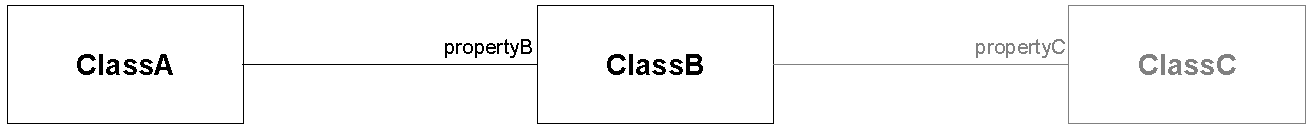
\includegraphics[width=1.00\textwidth]{figures/info/transitiveTypeImport.pdf}
	\caption{Transitive Import of Java Classes as a Model into DresdenOCL.}
	\label{fig:info:transitiveTypeImport}
\end{figure}

To import Java classes into DresdenOCL two possibilities exist:

\begin{enumerate}
	\item \code{*.class} files can be imported as a model. All directly referenced classes (either as types of properties and operations or their arguments) are imported as well. \textbf{Please be aware, that only byte code classes (\code{*.class}) and not source code classes \code{*.java} can be imported into DresdenOCL!}
	\item Alternatively, the path leading to the Java class to be imported can be declared in a text file matching to the file naming pattern \code{*.javamodel}. This alternative was implemented to support the import of Java classes referencing other external Java classes provided as \acs{JAR}s. An example for a \code{*.javamodel} text file is shown in Listing \ref{lst:javaModel}. The first line references the \code{JarClassProvider.class} that shall be imported as a model. The second line references a \acs{JAR} file that contains classes whose types are referenced in the \code{JarClassProvider.class}. Both, the class and the \acs{JAR} are referenced via relative \acs{URL}s from the directory where the \code{*.javamodel} file is located in the file system. Further lines of the \code{*.javamodel} text file could be used to reference additional \acs{JAR}s to be imported as well. Please be aware, that only referenced classes from the \acs{JAR}s are imported into DresdenOCL. Again, further classes are imported when required during \acs{OCL} parsing or evaluation.
\end{enumerate}

\begin{figure}[t]
\lstset{language=OCL, label={lst:javaModel}, caption={Example for a .javamodel File.}, captionpos=b}
\begin{lstlisting}
../bin/package1/package2/JarClassProvider.class
../lib/simple.jar
\end{lstlisting}
\end{figure}


\subsection{MDT UML Class Diagrams}

DresdenOCL allows to import UML class diagrams modelled with the \emph{\acf{Eclipse MDT}}. Typically, \acs{MDT} \acs{UML} models are stored as \acs{XMI} files matching to the naming pattern \code{*.uml}. Since many Eclipse-based modelling tools built on top of \acs{MDT} \acs{UML}, their models can be imported as well. Examples for such modelling tools are the \emph{\acf{GMF}} \acs{UML} class diagram editor and the \emph{Topcased} \acs{UML} class diagram editor.


\subsection{XML Schemas as Models}

DresdenOCL allows to import \acl{XSD}s (\acs{XSD}) as models. Typically, \acs{XSD}s are stored in \acs{XML} files matching to the naming pattern \code{*.xsd}.



\section{Supported Model Instances In Dresden OCL}
\label{sect:info:modelinstances}

DresdenOCL is adapted to and thus allows the import of multiple types of model instances. Which types of model instances are supported by DresdenOCL is documented in this section.


\subsection{EMF Ecore-Based Model Instances}

Besides the creation of meta-models or \acs{DSL}s, the \acf{EMF} allows the generation of simple model editors that can be used to model instances of the Ecore-based models created before. E.g., you can create a simple \acs{DSL} using \acs{EMF}. Afterwards you can model an instance of this \acs{DSL} using an Ecore-generated model editor. Now, you can import your \acs{DSL} as a model into DresdenOCL and you can parse \acs{OCL} constraints defined on your \acs{DSL}. To check these constraints on the created model instance, you have to import this instance into DresdenOCL as well.

Thus, DresdenOCL allows to import instances of Ecore-based models as model instances. Typically, the instances are stored as \acs{XMI} files that match to a file naming pattern that ends with the name of your Ecore model. E.g., if you modelled an \code{myDSL.ecore} and created an instance of this model via an Ecore-generated model editor, the instance matches to the naming pattern \code{*.mydsl}.

Besides complete models it can be useful to import single model instance elements into Dres\-den\-OCL when using DresdenOCL directly from another software application via its \acs{API}. How this is possible is documented in Subsection~\ref{sect:modelInstanceTypeAdaptation:addIMIElement}. For Ecore model instances, this mechanism can be used to add single \code{EObjects} to a model instance in DresdenOCL.


\subsection{Java Model Instances}

Java objects can be regarded as instances of model elements described in class diagrams or similar models. Thus, the import of Java objects as model instances for \acs{OCL} constraint interpretation is a common use case. DresdenOCL supports two possibilities to import Java objects into DresdenOCL.

\begin{figure}[t]
\lstset{language=Java, label={lst:info:javaModelInstance}, caption={Example for a ModelInstanceProviderClass programmed in Java.}, captionpos=b}
\begin{lstlisting}
public class ModelInstanceProviderClass {

  /**
   * @return A {@link List} of {@link Object}s that are part of the
   *         {@link IModelInstance}.
   */
  public static List<Object> getModelObjects() {

    List<Object> result;
    result = new ArrayList<Object>();

    Person person1;
    person1 = new Person();
    person1.setName("Person Unspecific");
    person1.setAge(25);
    result.add(person1);

    /* Add further elements ... */
		
    return result;
  }
}
\end{lstlisting}
\end{figure}

\begin{enumerate}
	\item It is possible to create a \code{ModelInstanceProviderClass} containing a static method called \code{getModelObjects()} that returns a \code{List} of \code{java.lang.Objects} that shall be imported as a model instance. Listing~\ref{lst:info:javaModelInstance} shows an example of such a \code{ModelInstanceProviderClass}.
	\item Similar to Ecore model instances, it is possible to add single \code{java.lang.Objects} to an existing model instance via DresdenOCL's \acs{API} at runtime as documented in Subsection~\ref{sect:modelInstanceTypeAdaptation:addIMIElement}.
\end{enumerate}


\subsection{XML Model Instances}

DresdenOCL supports to import \acs{XML} files as model instances. Although \acs{XML} files cannot contain executable code, their elements can be used as data to be verified by structural \acs{OCL} integrity constraints. Typically \acs{XML} files conform to the file name matching pattern \code{*.xml}.



\section{Summary}

This chapter documented which version of OCL is supported by DresdenOCL. Furthermore, supported types of models, and model instances were presented. The following chapter will explain how to install and use DresdenOCL.